%% We use `subfiles' package
\documentclass[preamble.tex]{subfiles}
\begin{document}


\clearpage

\chapter{Results}
\label{ch:results}


\section{QuickHull}
\label{sec:quickhull}

Throughout this chapter we will use a \name{Data Parallel Haskell} implementation of the QuickHull algorithm that computes the convex hull of a finite set of points in the plane. It derives its name from the QuickSort algorithm and similarly uses a divide and conquer approach.

The convex hull for a set of points in the plane can be visualised as a polygon formed by a rubber band stretched around the points. The smallest set of points forming the polygon that encloses all other points is called the convex hull.

The result of finding convex hull of a set of points can be seen on the right of Figure~\ref{fig:qh-result}. The same figure depicts the three steps of the sample run of QuickHull algorithm.

In the original recursive solution In each recursive step the algorithm finds

\begin{hscode}
quickHull_r :: [:Point:] -> Line -> [:Point:]

quickHull_r^ :: [:[:Point:]:] -> [:Line:] -> [:[:Point:]:]
\end{hscode}


\begin{figure}
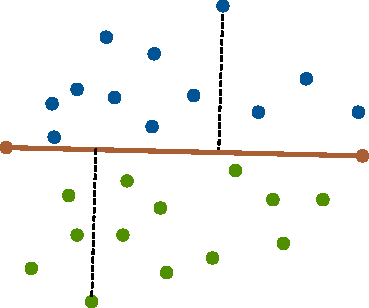
\includegraphics[width=0.3\textwidth]{img/Example-QuickHull-step1}~~~~~%
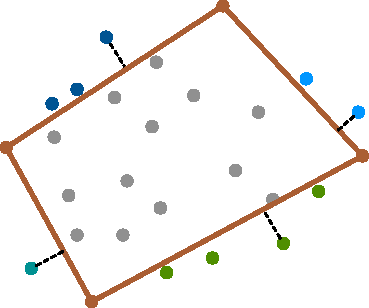
\includegraphics[width=0.3\textwidth]{img/Example-QuickHull-step2}~~~~~%
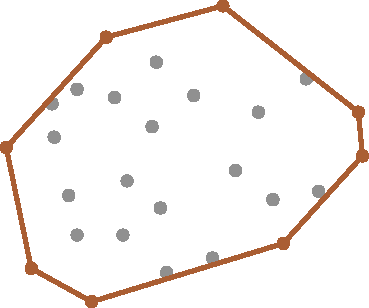
\includegraphics[width=0.3\textwidth]{img/Example-QuickHull-step3}%
\caption{A sample run of data parallel QuickHull algorithm.}
\label{fig:qh-result}
\end{figure}


\begin{hscode}[%
  caption={\label{fig:dph-qh}\name{Data Parallel Haskell} implementation of QuickHull.},
]
type Point = (Double, Double)
type Line  = (Point,  Point)

quickHull :: [:Point:] -> [:Point:]
quickHull points
  | lengthP points == 0 = points
  | otherwise
  = concatP [: quickHull_r points ends
                 | ends <- [: (minx, maxx), (maxx, minx) :] :]
  where
    xs   = [: x | (x, y) <- points :]
    minx = points !: minIndexP xs
    maxx = points !: maxIndexP xs

quickHull_r :: [:Point:] -> Line -> [:Point:]
quickHull_r points line@(start, end)
  | lengthP above == 0 = [:start:]
  | otherwise
  = concatP [: quickHull_r above ends
                 | ends <- [:(start, far), (far, end):] :]
  where
    -- Find relative distance from each point to the line
    distances = [: distance p line | p <- points :]
    -- Only keep points above the line
    above = [: p | (p,c) <- zipP points distances, c > 0.0 :]
    -- Find the point farthest from the line
    far = points !: maxIndexP distances

distance :: Point -> Line -> Double
distance (xo, yo) ((x1, y1), (x2, y2))
  = (x1 - xo) * (y2 - yo) - (y1 - yo) * (x2 - xo)
\end{hscode}



\subsection{The heart of QuickHull}

\subsection{Segmented FilterMax}

\subsection{Evaluation}

\begin{figure}
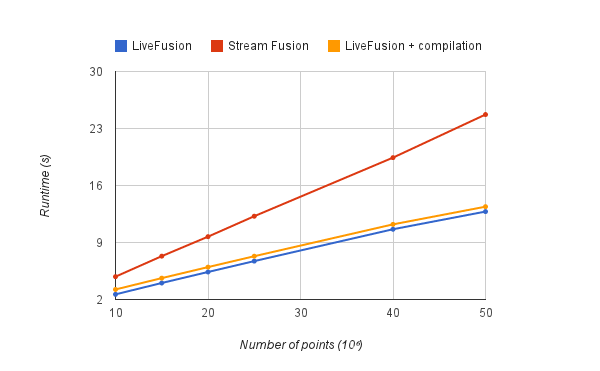
\includegraphics[center]{img/Eval-QuickHull}
\end{figure}

\begin{figure}
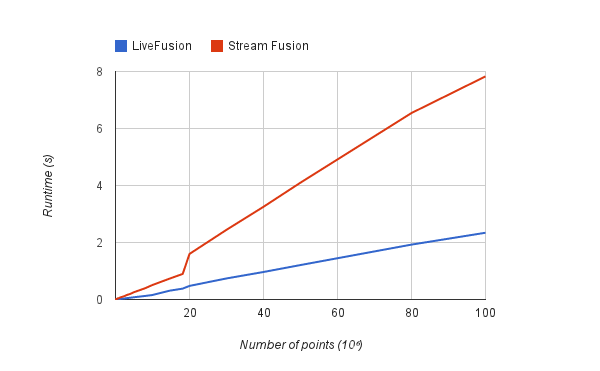
\includegraphics[center]{img/Eval-FarAndAboves}
\end{figure}

\begin{figure}
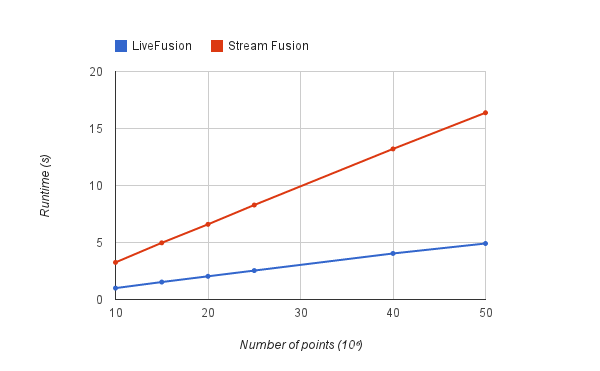
\includegraphics[center]{img/Eval-FarAndAboves-Overall}
\end{figure}

\clearpage
\section{Compilation time and amortisation}


\IfNotCompilingAll{\bibliography{bib}}

\end{document}